\section{Implementation and Evaluation}

In this section we present how we evaluated our approach. To do that, we extended the drone example with following scenarios, as illustrated by Figure~\ref{fig:simulation-scenario}: 

\begin{itemize}
    \item return to home/gliding: the return-to-home feature is executed whenever the drone bypasses a bad connection area (for instance, near to communication towers) in which the the drone loses connection with the pilot. This is a common safe procedure present in most drones currently. In the case of the medical payload delivery, this safety component becomes defiant since the bad connection can be transient and the drone could glide while waiting for the connection return. This way, we can maximize the chance of delivering the payload.  
    \item economy mode: if the battery reaches 15\%, then the drone enters in the economy mode, in which same sensors and the camera are switched off in order to save battery. However, by doing this, the pilot can loses the control of the drone, which may put in risk the medical payload. Therefore, the economy mode becomes defiant and should not occur during the medical delivery mission. 
\end{itemize}

\begin{figure*}[h]\centering
% 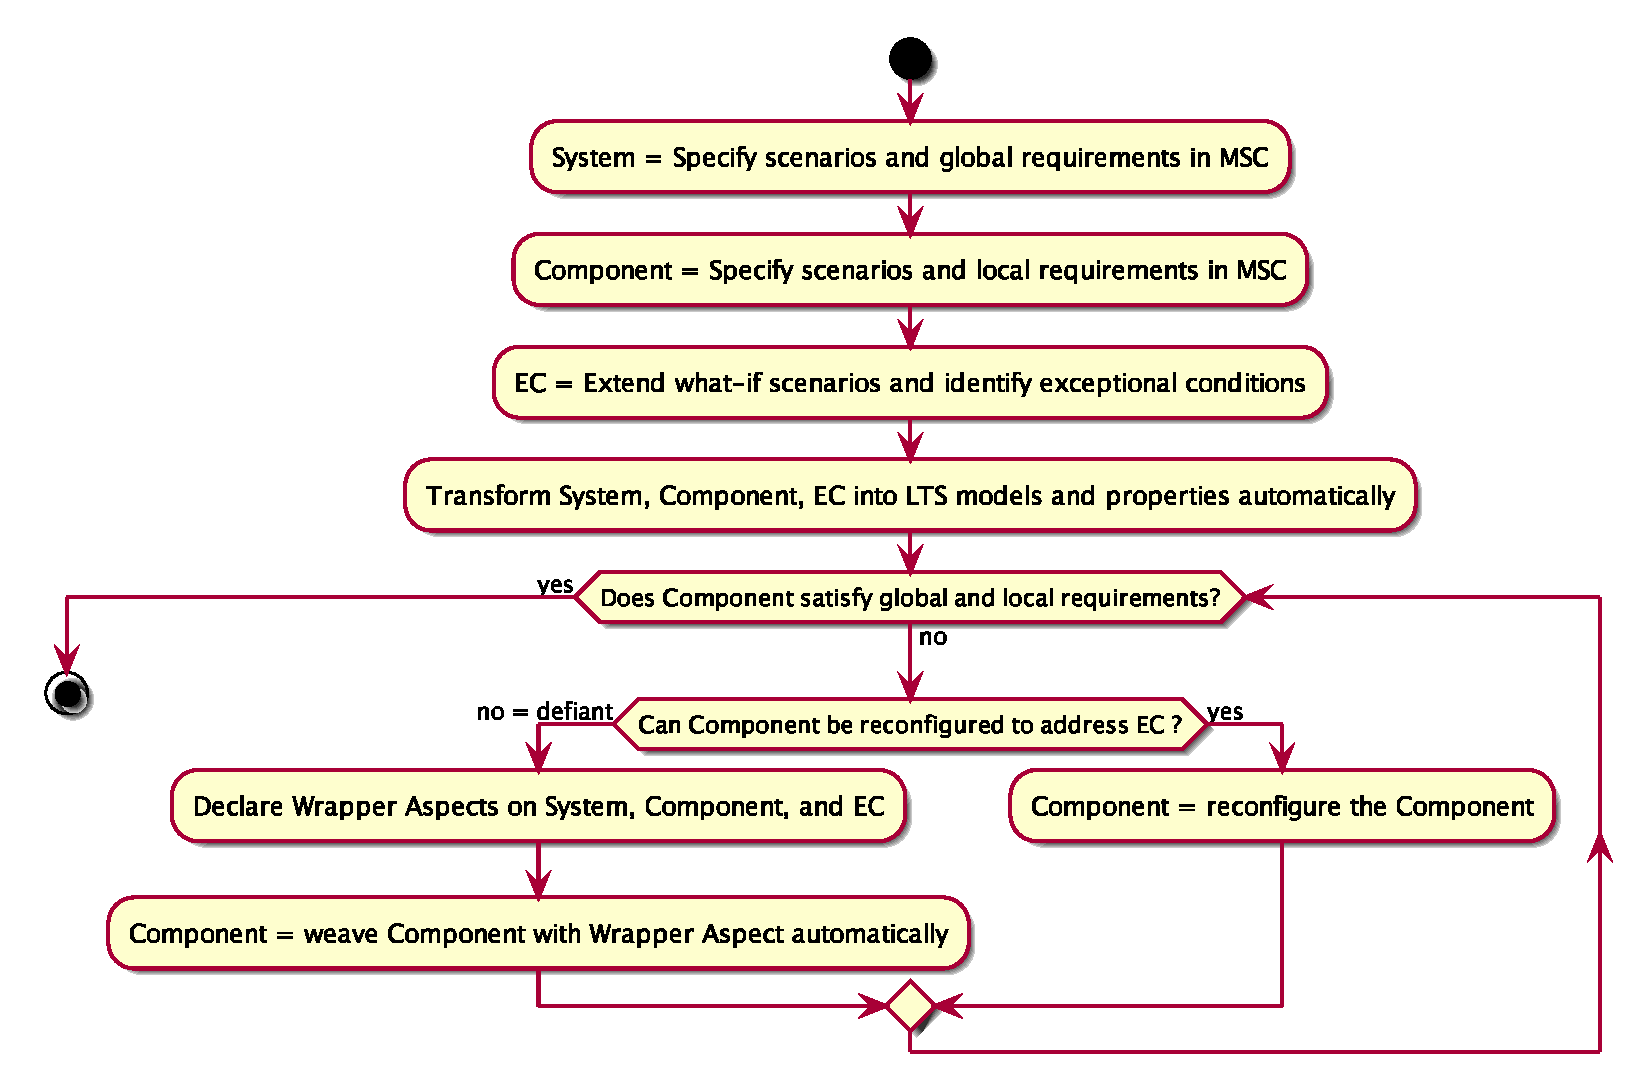
\includegraphics[width=0.9\columnwidth]{figures/activity.eps}
 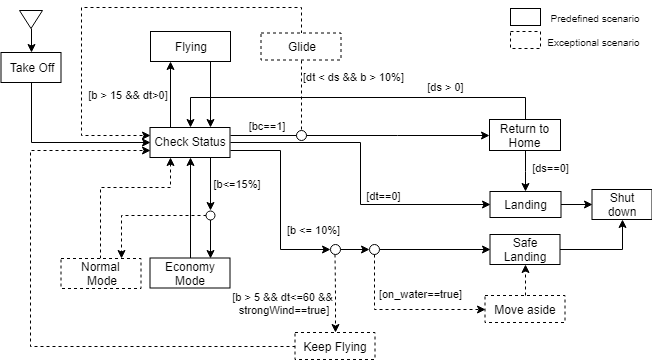
\includegraphics[width=0.7\textwidth]{figures/simulation-scenario.png}
 \caption{Simulation scenario}
 \label{fig:simulation-scenario}
 \vspace*{-0.5cm}
\end{figure*}

We implemented a prototype that simulates all behaviours indicated in Figure~\ref{fig:simulation-scenario}. Then we implemented a wrapper following the proposed approach described in section 3.1. In the simulator, the user can control either one or several drones at the same time. He/she can insert in a graphical user interface the source and destiny hospital, the communication towers, and draw the shape of the river. A snapshot of the simulator is depicted by Figure~\ref{fig:simulator}.   

\begin{figure}[h]\centering
% 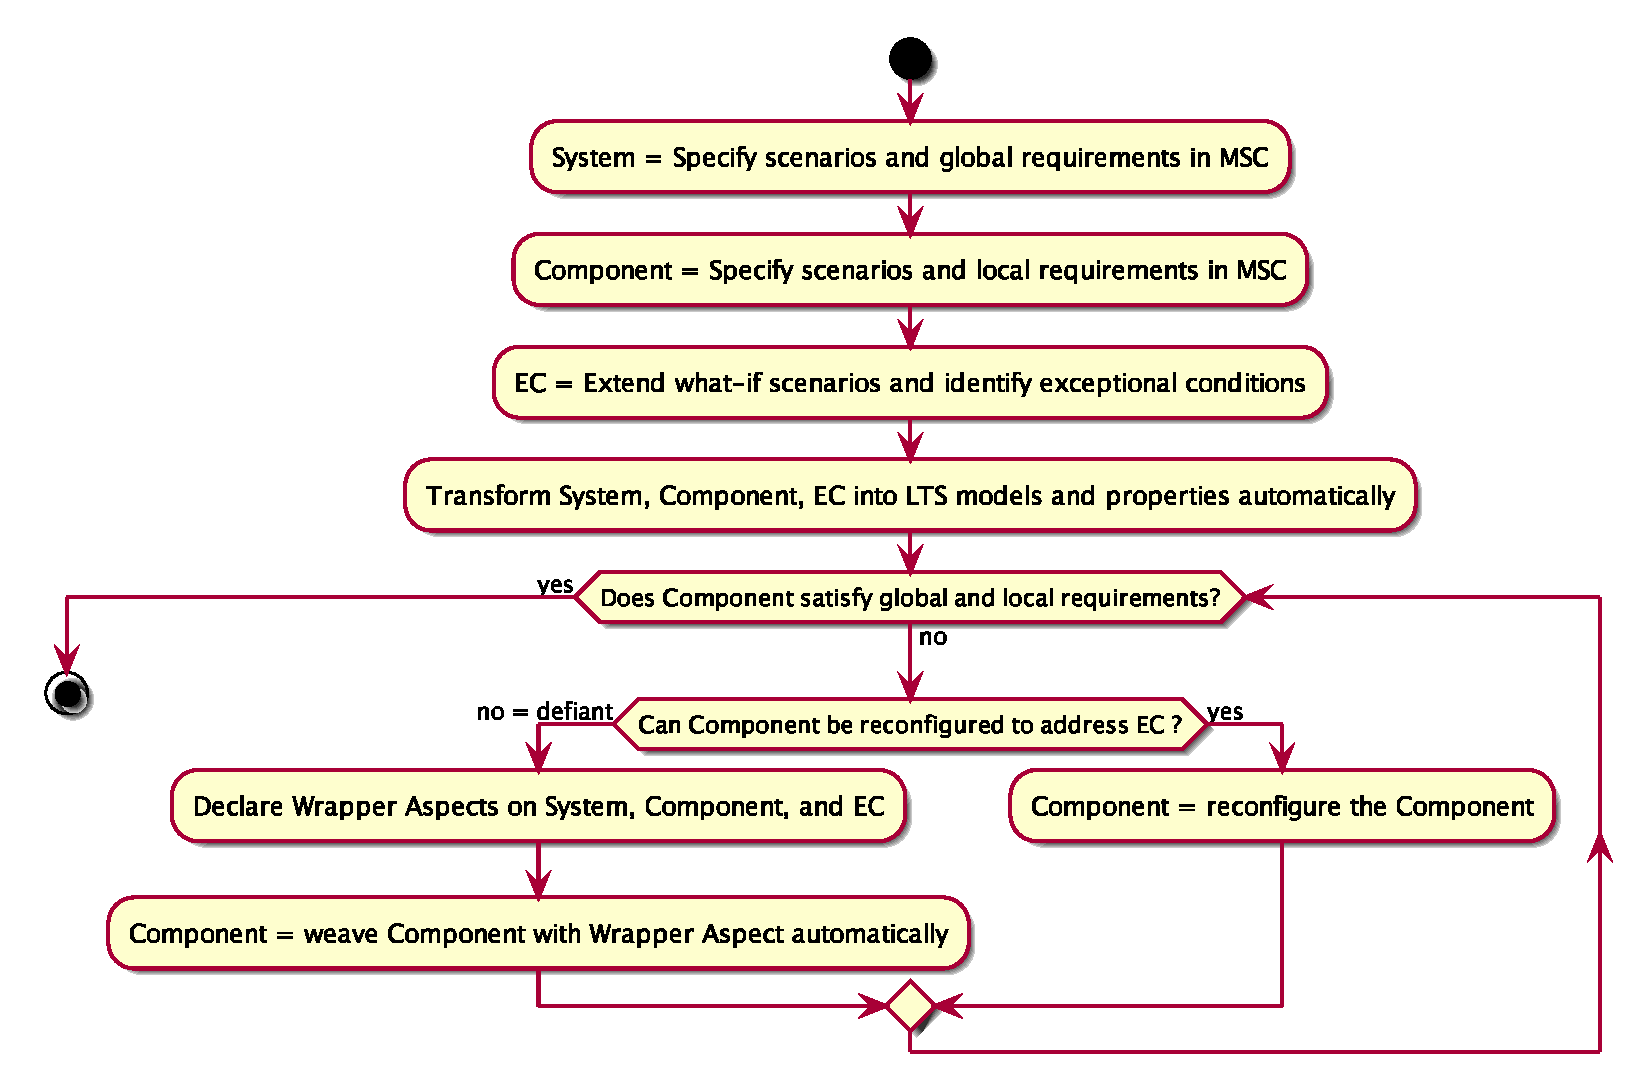
\includegraphics[width=0.9\columnwidth]{figures/activity.eps}
 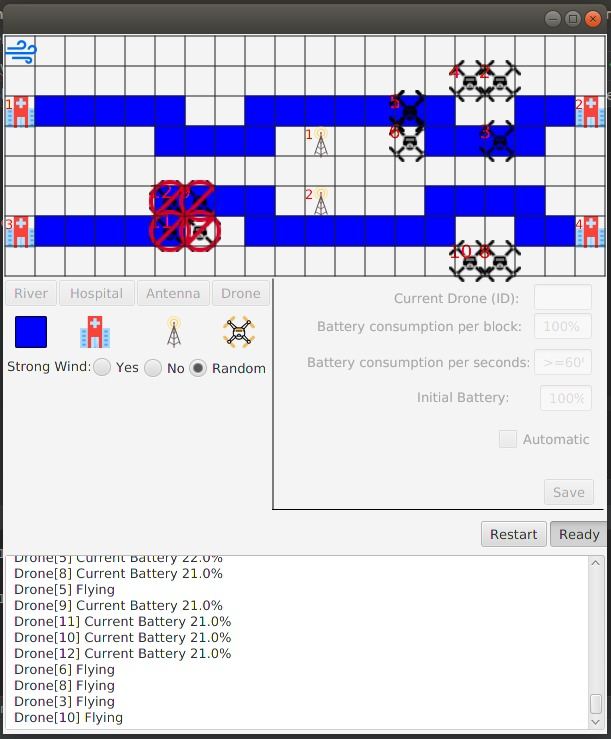
\includegraphics[width=0.4\textwidth]{figures/simulation.jpg}
 \caption{Screenshot of the simulation prototype}
 \label{fig:simulator}
 \vspace*{-0.5cm}
\end{figure}

We considered three criteria: (i) \textit{defiance removal}, which regards whether the drone behaves as expected with the wrapper; (ii) \textit{effectiveness}, regards when a fleet of drones is used to accomplish a mission; and (iii) conflict resolution, in which we discuss how our solution deals with when two or more components turn defiant at the same time. Each criterion is discussed as follows.

\subsection{Defiance removal}

Text to come...

\subsection{Effectiveness}

Text to come...

\subsection{Conflict resolution}

Text to come...


